\documentclass[11pt]{diazessay} % Font size (can be 10pt, 11pt or 12pt)

\usepackage{amsmath}
\usepackage{parskip}
\usepackage{graphicx}
\usepackage{amsthm}
\usepackage{tikz-cd}
\usepackage{mathtools}

\usetikzlibrary{babel}

\newtheorem{definition}{Definición}
\newtheorem{lemma}{Lema}
\newtheorem{proposition}{Proposición}

\DeclareMathOperator{\R}{\mathbb{R}}
\DeclareMathOperator{\im}{\textrm{im}}

\title{\textbf{La fibración de Hopf} \\ {\Large\itshape vista desde la geometría diferencial}} % Title and subtitle

\author{\textbf{David Lozano Campillo} \\ \textit{Universidad de Murcia}} % Author and institution

\date{\today} % Date, use \date{} for no date

\begin{document}

\maketitle % Print the title section

\begin{center}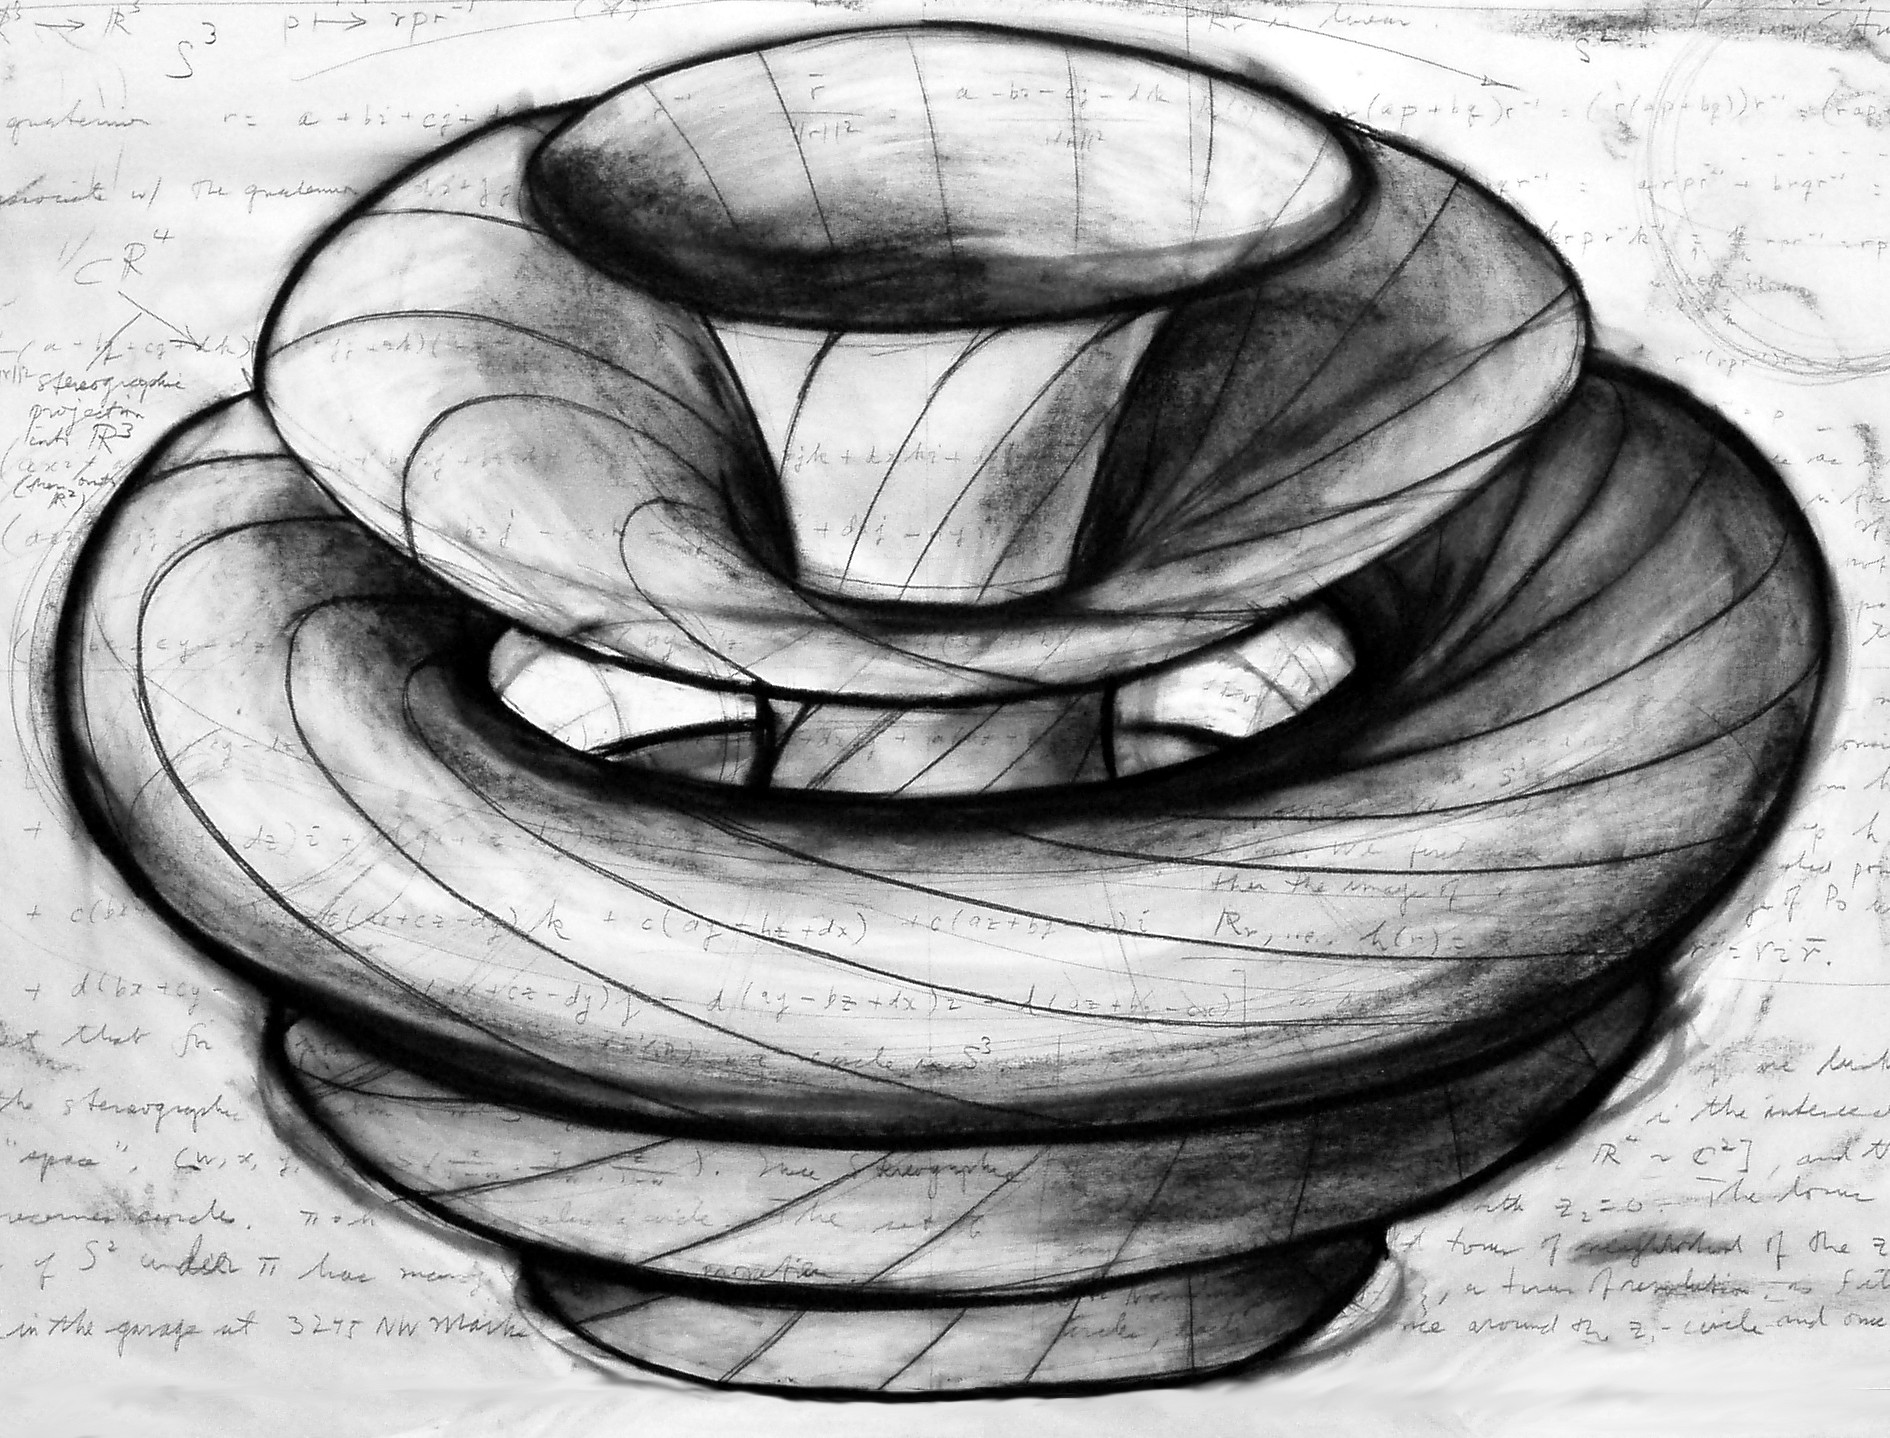
\includegraphics[width=8cm]{Figures/tsai.jpeg}\end{center}
\vspace{1cm}

\begin{abstract}

\end{abstract}

\hspace*{3.6mm}\textit{Keywords:} lorem, ipsum, dolor, sit amet, lectus % Keywords

\vspace{30pt}


\section*{Introducción}

La fibración de Hopf es una poderosa herramienta para poder visualizar la 3-esfera $S^3$, una superficie de 3 dimensiones en $\R^4$, como fibras de la 2-esfera. Para poder describirla de forma adecuada, debemos introducir el concepto de cuaterniones. El concepto de cuaternión fue descubierto por William Rowan Hamilton cuando buscaba una manera sincilla de descibir rotaciones en $\R^3$ al igual que los números complejos describen fácilmente una rotación en el plano $\R^2$ mediante la multiplicación.

Definimos los cuaterniones $\mathbb{H}$ como el conjunto de puntos de la forma $a+bi+cj+dk$, donde $ij=jk=ki=1$ y $ji=kj=ik=-1$, con el p. Dado un cuaternión $r=a+bi+cj+dk$, definimos su conjugado como $\overline{r}=a-bi-cj-dk$, y la norma como $|r|^2 = r\overline(r) = a^2+b^2+c^2+d^2$. Tenemos por lo tanto que el inverso de un cuaternón $r$ viene dado por $r^{-1}=\frac{\overline{r}}{|r|^2}$.

Un cuaternión $r$ define una aplicación $R_r:\R^3\to\R^3$ de la siguiente manera: identificando $\R^3$ como el conjunto de cuaterniones imaginarios, definimos $R_r(p) = rpr^{-1}$. Se puede comprobar que dicho producto es también un cuaternión imaginario, luego podemos identificarlo con un punto de $\R^3$

Claramente la aplicación $R_r$ conserva la norma, pues $|rpr^{-1}|=|r||p||r^{-1}|=|p||r||r|^{-1}=|p|$. Además, se puede verificar que $R_{kr} = R_r$ siendo $k$ un número real, luego suponemos a partir de ahora que $r$ tiene norma 1. Es fácil comprobar que si $r=a+bi+cj+dk$, entonces $(b,c,d)$ es un autovector de $R_r$ con autovalor 1. Por lo tanto, $R$ es una rotación en el espacio euclídeo $\R^3$ y su eje viene determinado por el subespacio generado por $(b,c,d)$. El ángulo se puede calcular fácilmente tomando un vector $w$ perpendicular a $(b,c,d)$, por ejemplo $(c,-b,0)$ si al menos algún $b,c$ es distinto de cero, o $(1,0,0)$ en el otro caso. Aplicando la fórmula
\[\cos\theta = \frac{wR_rw}{|w|^2}\]
obtenemos que $\theta = 2\arccos(a)$.

Vamos a definir un punto distinguido en la 2-esfera, $P_0=(1,0,0)=i$ en nuestra identificación. Entonces dado un punto en la 3-esfera, por la discusión anterior vemos que dicho cuaternión define una rotación $R_r$, y definimos entonces la fibración de Hopf: $\pi:S^3\to S^2$ como $\pi(r)=ri\overline{r}$.

\begin{definition}
    Dado $r=a+bi+cj+dk\in S^3$, definimos la fibración de Hopf como la aplicación $\pi:S^3\to S^2$
    \[\pi(r)=ri\overline{r}=(a^2+b^2-c^2-d^2)i+2(ad-bc)j+2(bd-ac)k\]
\end{definition}

Calculemos la fibra del punto $(1,0,0)=i$:

\begin{proposition}
    $\pi^{-1}(i)=\{\cos\theta+i\sin\theta\}_{0\leq\theta\leq 2\pi}$
\end{proposition}
\begin{proof}
    Suponemos que $r=a+bi+cj+dk\in S^3$ tal que $\pi(r)=i$. Tenemos entonces que $a^2+b^2+c^2+d^2=1$, $a^2+b^2-c^2-d^2=1$. Restando la segunda a la primera obtenemos que $c^2+d^2=0$, luego $c=d=0$. Tenemos por lo tanto $a^2+b^2=1$, lo que implica el resultado que queremos demostrar.
\end{proof}

Tenemos por lo tanto que para un punto $p$, la fibra $\pi^{-1}(p)$ consiste en el conjunto de rotaciones que llevan $p$ a $i$. Dados dos puntos en $S^2$, el eje de una rotación que lleva un punto a otro está en el gran círculo que bisecta el arco entre ambos puntos. Por lo tanto, dada una rotación que lleva $p$ a $i$ por el cuaternión $r_0$, el conjunto de rotaciones que llevan $p$ a $i$ viene dado por el conjunto
\[\pi^{-1}(p) = \{r_0e^{i\theta}\}_{0\leq\theta\leq 2\pi}.\]

También podemos observar esto viendo que si $s$ es un elemento de la fibra, entonces $sis^-1=p=r_0i\overline{r_0}$, luego $(s^-1r_0)i\overline{(\overline{s}r_0)}=i$, es decir, $\overline{s}r_0$ está en la fibra de $i$. Claramente $\pi^{-1}(i)=\{\cos\theta+i\sin\theta\}_{0\leq\theta 2\pi}$, y por lo tanto $s=r(\cos\theta+i\sin\theta)$.
Hemos visto que las fibras de la aplicación de Hopf son circunferencias, y además, tenemos claramente que $\pi(S^3)=S^2$.

\begin{center}
    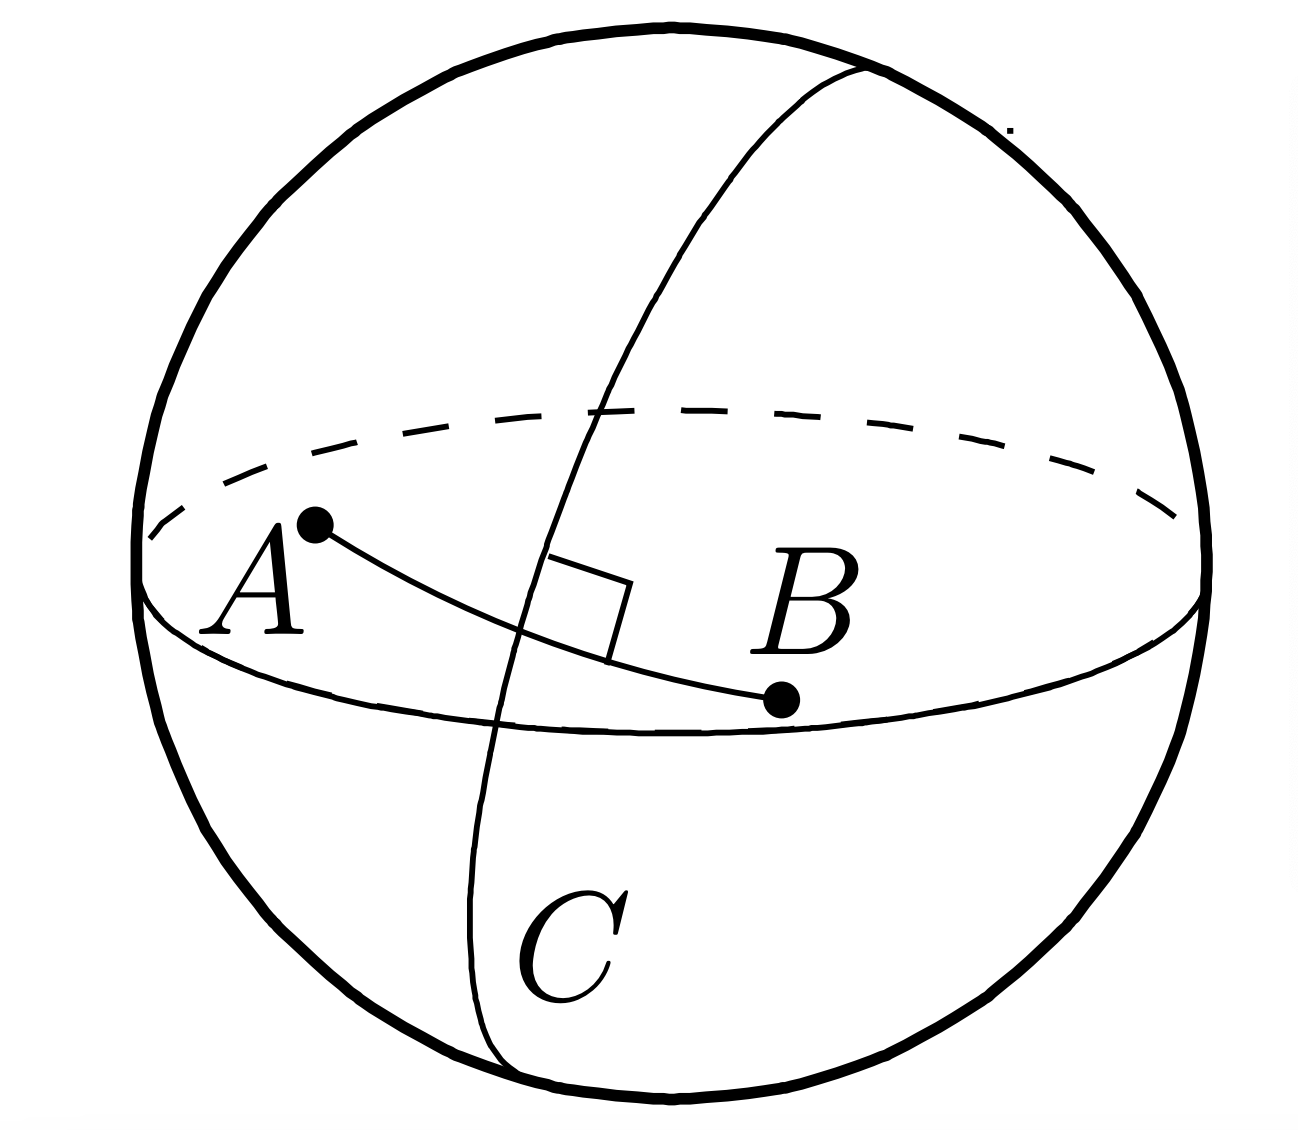
\includegraphics[width=4cm]{Figures/bisectriz.png}
\end{center}

\section*{Visualizando la fibración de Hopf}

Sabemos que las fibras de la fibración de Hopf son circunferencias, pero, ¿cómo las visualizamos al estar dentro de un espacio 4-dimensional? Usamos la herramienta más socorrida al estudiar las esferas, y conocida por cualquier matemático, sea geómetra o no: la proyección estereográfica. Esta proyección (en $S^2$) hace corresponder a un punto de la esfera (a excepción de un punto distinguido, que en nuestro caso será el ``polo norte'', $(0,0,1)$) el punto de intersección de la recta que pasa por el polo y por el plano generado por $(1,0,0)$ y $(0,1,0$).

Una propiedad muy importante de la proyección estereográfica es que lleva circunferencias (que no pasan por el polo norte) a circunferencias en el plano. Si una circunferencia pasa por el polo norte, es proyectada a una recta. En el caso de la $S^3$, vamos a tomar como polo norte el punto $(1,0,0,0)$. Sabemos por la sección anterior que las fibras de $\pi$ son circunferencias, luego son proyectadas a circunferencias, a excepción de si pasan por el polo norte, que son poryectadas en recta. Denotemos $s$ por dicha proyección estereográfica. Entonces es claro lo siguiente:

\begin{itemize}
    \item $s\circ\pi^{-1}((1,0,0))$ es el eje $x$, ya que el punto $(1,0,0,0)$ (la rotación identidad) se encuentra en la fibra, y por tanto $s$ proyecta dicha circunferencia al eje $x$.
    \item $s\circ\pi^{-1}((-1,0,0))$ es el circulo unidad en el plano $y,z$. Esto se debe a que $\pi^{-1}((-1,0,0))=\{ke^{i\theta}\}_{0\leq\theta\leq 2\pi}=\{j\sin \theta + k\cos \theta\}_{0\leq\theta\leq 2\pi}$
    \item Para cualquier otro punto $P$ distinto, $s\circ\pi^{-1}(P)$ es una circunferencia que interseca el plano $y,z$ en dos puntos, uno fuera y otro dentro del círculo unidad. Esto se puede comprobar viendo que si $P=(p_1,p_2,p_3)$ es dicho punto, entonces $r_1=\sqrt{\frac{1+p_1}{2}}(1-p_3j+p_2k)$ es un cuaternión que describe una rotación que lleva $P$ a $i$. Por lo tanto, la fibra viene dada por $r_1e^{i\theta}$. Poniendo $r_1=a+bj+ck$ para simplificar los cálculos, podemos expresar la fibra como
          \[a\cos\theta + a\sin\theta i + (b\cos\theta + c\sin\theta)j + (c\cos\theta -b\sin\theta)k.\]
          Usando ahora la descipción de la proyección estereográfica como \[(w,x,y,z)\mapsto\left(\frac{x}{1-w},\frac{y}{1-w},\frac{z}{1-w}\right)\]
          tenemos que dicha proyección viene dada por
          \[\left(\frac{a\sin\theta}{1-a\cos\theta},\frac{b\cos\theta+c\sin\theta}{1-a\cos\theta},\frac{c\cos\theta-b\sin\theta}{1-a\cos\theta}\right).\]
          Esta proyección interseca al plano $y,z$ en dos puntos, cuando $\theta=0,\pi$, y por tanto los dos puntos son $(0,\frac{b}{1-a},\frac{c}{1-a})$ y $(0,\frac{-b}{1+a},\frac{-c}{1+a})$. Se puede comprobar fácilmente que uno de ellos tiene norma menor que 1 y otro normal mayor que 1, sustituyendo $a,b,c$ por sus valores correspondientes y que $(p_1,p_2,p_3)$ tiene norma 1. Por lo tanto, $s\circ\pi^{-1}(P)$ está enlazado con el círculo unidad en el plano $y,z$. Además, el eje $x$ pasa por el interior de este círculo, ya que el plano de $s\circ\pi^{-1}(P)$ no puede contenerlo (si no, las dos fibras se intersecarían y sabemos que son disjuntas.)
\end{itemize}

\section*{Sumersiones riemannianas}

Viendo la fibración de Hopf desde el punto de vista de la geometría de variedades de Riemann, es fácil comprobar que es una sumersión. Recordemos la definición de sumersión: $\pi:M\to N$ es una sumersión diferenciable si es una aplicación diferenciable entre las variedades $M$ y $N$ y además su diferencial es sobreyectiva en todo punto, es decir, tiene rango máximo. Haciendo las cuentas con cuaterniones, podemos ver que la fibración de Hopf tiene la siguiente forma:
\[\pi(w,x,y,z) = (w^2 + x^2 - y^2 - z^2, 2(wz + xy), 2(xz - wy))\]

Si consideramos la aplicación como una aplicación $H:\R^4\to \R^3$, y calculamos el jacobiano de dicha aplicación para un $p=(w,x,y,z)$:
\[
    dH_{p}=\begin{pmatrix}
        2w  & 2x & -2y & -2z \\
        2z  & 2y & 2x  & 2w  \\
        -2y & 2z & -2w & 2x
    \end{pmatrix}
\]

Tenemos que es claramente de rango 2, ya que el valor absoluto del menor formado con las tres primeras columnas vale $|8y|$, el formado con las tres últimas vale $|8x|$, el formado con la primera, cuarta y tercera vale $|8w|$ y el formado con la cuarta, primera y segunda vale $|8z|$. Como restringimos la aplicación a la $S^3$, ninguno de los valores se anula simultáneamente y por lo tanto $dH_p$ tiene rango 3 para todo punto $p\in S^3$.

Usaremos ahora el siguiente lema:

\begin{lemma}
    Sea $U\subseteq \R^{n+1}$ un subespacio $n$-dimensional, y $T:\R^{n+1}\to\R^n$ una aplicación lineal con rango máximo. Si $V\subseteq \R^n$ es un subespacio $n-1$-dimensional que contiene a $T(U)$, la restricción $T|_U:U\to V$ tiene rango $n-1$.
\end{lemma}
\begin{proof}
    Usamos el teorema del rango-nulidad en $T$ y en $T|_U$, teniendo que
    \begin{align*}
        \dim(\ker T)   & = \dim(\R^{n+1}) - \dim(\im T) \\
        \dim(\im T|_U) & = \dim(U) - \dim(\ker T|_U)
    \end{align*}

    Si $\dim(\im T)=n$, entonces $\dim(\ker T)=1$. Como $\ker T|_U\subseteq \ker T$, tenemos que $\dim(\ker T|_U)\leq \dim(\ker T)=1$. Por lo tanto, tenemos que $\dim(U)-\dim(\ker T|_U) \geq n-1$, y por lo tanto $\dim(\im T|_U)\geq n-1$. Como $\im T|_U\subset V$ y $\dim V = n-1$, tenemos que $\dim(T_U)\leq n-1$. Por lo tanto, tenemos que $\dim(T|_U)=n-1$.
\end{proof}

Como $S^3$ es una subvariedad de $R^4$, la restricción de la aplicación $H:\R^4\to \R^3$ (que es diferenciable), que es la composición con la inclusión $S^3\hookrightarrow\R^4$ es diferenciable. Además, como $\im(\pi|_{S^3})=\im\pi\subseteq S^2$, tenemos que la restricción de $H|_{S^3}$ al codominio es diferenciable \cite[Corolario 1.29]{Oneill_1983}

Tenemos que $\dim(T_pS^3)=3, \dim(T_pS^2)=2$ y que $dH_p$ tiene rango máximo, luego por el lema anterior, la restricción de $H|_{S^3}$ tiene rango 2. Por lo tanto, $\pi$ es una sumersión. También podemos comprobar que es un haz de fibras. Para ello demos primero la definición:

\begin{definition}
    Sea $B$ un espacio conexo, y $p:E\to B$ una aplicación continua del \textit{espacio total} $E$ al \textit{espacio base} $B$. Decimos que $p$ es un haz de fibras con fibra $F$ si $p$ es sobreyectiva y para cada $x\in B$,
    \begin{enumerate}
        \item $p^{-1}(x)$ homeomorfo a $F$ y
        \item eiste un entorno $U_x\subseteq B$ de $x$ y un homeomorfismo $\Psi_{U_x}:p^{-1}(U_x)\to U_x\times F$, llamada una trivialización local de $E$ sobre $U$. En otras palabras, el siguiente diagrama conmuta:
              \[
                  \begin{tikzcd}
                      p^{-1}(U_x) \arrow[rr, "\Psi_{U_x}"] \arrow[rd, "p"] & & U_x\times F \arrow[ld, "\textrm{proj}_1"] \\
                      & U_x &
                  \end{tikzcd}
              \]
    \end{enumerate}

    Si $E$, $B$, $F$ son variedades diferenciables y $\Psi_{U_x}$ y $p$ son difeomorfismos, entonces decimos que $p$ es un haz de fibras diferenciable.
\end{definition}

Intuitivamente, que la fibración sea un haz de fibras significa que para un entorno suficientemente pequeño, la fibra de dicho entorno es homeomorfo a un cilindro. El fibrado no es trivial (que sea trivial signific que $U_x=B$), ya que, tal y como hemos visualizado, la fibración produce torsión. El siguiente lema nos va a asegurar que $\pi$ es un haz de fibras:

\begin{lemma}[Lema de Ehresmann]
    sea $F:M\to N$ un a aplicación entre variedades diferenciables tal que
    \begin{enumerate}
        \item $F$ es una sumersión sobreyectiva
        \item $F$ es una aplicación propia
    \end{enumerate}
\end{lemma}

Como $\pi$ es una sumersión, sobreyectiva, y $S^3$ es compacto (luego automáticamente $\pi$ es propia), tenemos que define un haz de fibras, que podemos representar de la siguiente manera:
\[S^1\hookrightarrow S^3\to S^2.\]

Visto esto, cabe preguntarnos: ¿se generaliza la fibración de Hopf a más dimensiones? La respuesta es que si, pero solo en tres casos más, hasta dar un total de cuatro fibrados:
\begin{align*}
    S^0 & \hookrightarrow S^1 \to S^1    \\
    S^1 & \hookrightarrow S^3 \to S^2    \\
    S^3 & \hookrightarrow S^7 \to S^4    \\
    S^7 & \hookrightarrow S^{15} \to S^8
\end{align*}

Este es conocido como el teorema de la invarianza uno de Hopf o teorema de Adams \cite{adams}.

Hasta ahora solo hemos considerado conceptos diferenciales de la fibración de Hopf, sin tener en cuenta la métrica inducida por la métrica euclídea que tienen $S^2$ y $S^3$. Veremos que la fibración de Hopf es una \textit{sumersión riemanniana}. Tal y como la define O'Neill en \cite{oneill_1966}, si suponemos que las fibras son subvariedades riemannianas (lo cual es claro ya que son $S^1$ inmersas en $S^3$), descomponemos su espacio tangente como la suma directa del espacio tangente a las fibras con su ortogonal. Dado $p:E\to B$, y denotando por $E_q=p^{-1}(q)$ la fibra de $q$, tenemos que
\[T_qE = T_q(E_q)\oplus T_q(E_q)^\bot\]
Dado un vector, llamamos parte \textit{vertical} de ese vector como la proyección sobre el subespacio tangente a la fibra, y parte horizontal como la proyección al ortogonal.

\begin{definition}
    Decimos que $p:E\to B$ es una sumersión riemanniana si para cada $q\in E$ se tiene que $d\pi_q$ conserva la longitud de los vectores horizontales
\end{definition}

Veamos cual es el espacio horizontal y vertical en el punto de una fibra. Sea $\psi:(-\epsilon,\epsilon)\to S^3$ curva en la fibra de un punto $p\in S^3$, esto es, $\pi(\psi(t))=p$, y sea $\psi_0=\psi(0)$. Tenemos entonces que $\psi$ es de la forma $\psi(t)=\psi_0e^{i\alpha(t)}$, donde $\alpha(0)=0$. Derivando cuando $t=0$ tenemos que
\[\psi'(0)=\psi_0(e^{i\alpha})'(0)=\psi_0 i\alpha'(0)\]
Por lo tanto el espacio vertical a la fibra en $\psi_0$ viene dado por
\[\mathcal{V}_{\psi_0}=\psi_0i\R.\]
Y el espacio horizontal $\mathcal{H}_{\psi_0}$ viene entonces dado por el ortogonal al espacio anterior. Como los vectores verticales son parte del espacio tangente del espacio total ($S^3$), también deben ser ortogonales a $\psi_0$.

Vemos a continuación el primer resultado que relaciona la fibración de Hopf con la métrica:

\begin{proposition}
    La restricción de $d\pi_{\psi_0}$ a $\mathcal{H}_{\psi_0}$ preserva la métrica, salvo un factor de 4: para todo $v, w\in\mathcal{H}_{\psi_0}$ se tiene que
    \[\langle d\pi_{\psi_0}(v), d\pi_{\psi_0}(w)\rangle = 4\langle v,w\rangle.\]
\end{proposition}
\begin{proof}
    Comuptamos la diferencial de $\pi$: para cada vector tangente $v\in T_{\psi_0}S^3$ existe una curva $\gamma:(-\epsilon,\epsilon)\to S^3$ tal que $\gamma(0)=\psi_0$ y $\gamma'(0)=v$. Aplicando la regla del producto
    \[d_{\psi_0}\pi(v)=(\pi\circ\gamma)'(0)=\gamma'(0)i\overline{\gamma(0)}+\gamma(0)i\overline{\gamma'(0)} = vi\overline{\psi_0}+\psi_0i\overline{v}\]

    Calculamos primero la diferencial en $\psi_0=1$. Tenemos entonces que $v\in \mathcal{H}_1$ si y solo si $v \in \mathrm{span} \{j,k\}$. Por lo tanto tenemos que para $v\in\mathcal{H}_1$,
    \[d_1\pi(v)=vi+i\overline{v} = 2vi\]

    Sea ahora $\psi_0$ un punto arbitrario de $S^3$, y $\in \mathcal{H}_{\psi_0}$. Tenemos por lo tanto una curva $\gamma(0)=\psi_0$ y $\gamma'(0)=v$. Definiendo $\tilde{\gamma}\coloneqq \overline{\psi_0}\gamma$. Esto es, $\gamma = \psi_0\tilde{\gamma}$. Entonces $\tilde{\gamma}$ es una curva en $S^3$ que pasa por el punto 1. Por lo tanto $\tilde{v}\coloneqq \tilde{\gamma}'(0)\in T_1S^3$. Tenemos entonces que
    \[\pi\circ\gamma=\gamma i\overline{\gamma} = \psi_0(\pi\circ\tilde{\gamma})\overline{\psi_0}.\]
    Obtenemos por lo tanto que
    \[d_{\psi_0}(v) = (\pi\circ\gamma)'(0)=\psi_0(\pi\circ\tilde{\gamma})'(0)\overline{\psi_0}= \psi_0d_1\pi(\overline{v})\overline{\psi_0}.\]
    Además tenemos que \[\tilde(v)=\tilde{\gamma}'(0)=\overline{\psi_0}\gamma'(0)=\overline{\psi_0}v.\]
    En particular, $\tilde{v}\in\mathcal{H}_1$. Por lo tanto
    \[d_{\psi_0}(v) = \psi_0d_1\pi(\overline{v})\overline{\psi_0} = \psi_02\tilde{v}i\overline{\psi_0} = 2vi\overline{\psi_0}.\]
    La multiplicación por cuaterniones unitarios es una isometría: si $\psi\in S^3$, entonces $\langle \psi x, \psi y\rangle = \langle x\psi, y\psi\rangle = \langle x, y\rangle$. Tenemos entonces el resultado que buscábamos.

    Tenemos que redefinir entonces ligeramente la definición de la fibración de Hopf para corregir ese factor de 4, con el objetivo de que la fibración sí que sea una sumersión riemanniana: definimos la fibración como la aplicación $r\mapsto \frac{1}{2}ri\overline{r}$, que lleva la $S^3(1)$ a la $S^2(\frac{1}{2})4$. En este caso, es fácil comprobar que sí que es una isometría, ya que $d\pi_1(v) = \frac{1}{2}2vi$ para vectores $v\in\mathcal{H}_1$, y se generaliza de manera inmediata para vectores arbitrarios siguiento el mismo razonamiento que antes.

    \section*{Cilindros y toros de Hopf}

    Sea ahora $\gamma:[0,L]|\to S^2$ una curva parametrizada por el arco. Tenemos entonces que la fibra de esta curva por la fibración de Hopf es un cilindro (es una familia de círculos). Para parametrizar este cilindro, comenzamos con una cuva \textit{levantamiento} de $\gamma$, que denominaremos $\psi_0:[0,L]\to S^3$ y que proyecta sobre $\gamma$ por la fibración de Hopf: $\pi\circ\psi_0=\gamma$. Tal y como hemos generado las fibras de Hopf en un punto anteriormente, tenemos que la parametrización del cilindro viene dada por \[f_0:[0,L]\times \mathbb{Z}/2\pi\mathbb{Z}\to S^3\quad (t,\theta)\mapsto \psi_0(t)e^{i\theta}.\] Buscamos una parametrización isométrica, luego las derivadas parciales deben tener norma 1 y ser ortogonales. Calculemoslas:
    \begin{align*}
        \frac{\partial f_0}{\partial\alpha} & = \psi_0 e^{i\alpha} i \\
        \frac{\partial f_0}{\partial t} & = \psi_0'(t)e^{i\alpha}
    \end{align*}

    Claramente $|\frac{\partial f_0}{\partial\alpha}| = |\psi_0| = 1$, y que $\frac{\partial f_0}{\partial\alpha}\in\mathcal{V}_{\psi_0}$, luego para que ambas derivadas parciales sean ortogonales, debemos tener que $ \frac{\partial f_0}{\partial t}\in \mathcal{H}_{\psi_0(t)}$. Esto es lo que se llama un levantamiento horizontal. Este levantamiento se puede obtener como la curva integral de las proyecciones del vector que deseamos a $\mathcal{H}_{\psi_0(t)}$. La existencia de curvas integrales siempre es cierta localmente, refiérase para una demostración por ejemplo a \cite[Teorema 9.12]{Lee_2003}. Tenemos entonces por la Proposición 2 que
    \[|\psi_0| = \frac{1}{2}|d\pi(\psi')_\psi| = \frac{1}{2} |(\pi\circ\psi)'| = \frac{1}{2} |\gamma'|\]

    En vez de reducir el radio de la $S^2$, reescalamos el parámetro $t$ a $t/2$, obteniendo entonces el siguiente resultado:

    \begin{proposition}
        Sea $\gamma:[0,L/2]\to S^2$ tal que $|\gamma'|=2$, y sea $\psi$ un levantamiento horizontal a la $S^3$. Tenemos entonces que $f:[0,L/2]\times \mathbb{Z}/2\pi\mathbb{Z}\to S^3,\quad (t,\alpha)\mapsto \psi(t)e^{i\alpha}$ es una parametrización isométrica del cilindro de Hopf definido por $\gamma$.
    \end{proposition}

    Por lo tanto, mientras que en $R^3$ un toro nunca puede ser isométrico a un cilindro (ya que su curvatura de Gauss es no nula), cualquier toro de Hopf \textit{sí} que es isométrico a un cilindro.

\end{proof}


\bibliographystyle{plain}
\bibliography{sample.bib}

\end{document}
